\documentclass{ximera}
\graphicspath{
{./}
{volumes/}
{arclengths/}
{centroids/}
{techniques/}
{applications/}
{series/}
{powerseries/}
{odes/}
{lessons/}
}
\usepackage{booktabs}

\newcommand{\bigmath}[1]{$\displaystyle #1$}
\newcommand{\choicebreak}{}
\newenvironment{type}{}{}
\newenvironment{notes}{}{}
\newenvironment{keywords}{}{}
\newcommand{\offline}{}
\newenvironment{comments}{\begin{feedback}}{\end{feedback}}
\newenvironment{multiplechoice}{\begin{multipleChoice}}{\end{multipleChoice}}
\title{Exercises: Disks and Washers}
\author{Philip T. Gressman}

\begin{document}
\begin{abstract}
Exercises for the disk and washer methods.
\end{abstract}
\maketitle

\begin{exercise}
The region $0 \leq y \leq \sqrt{x}$ with $x \leq 1$, shown below, is revolved around the $x$-axis. Use the disk method to find the volume of the solid of revolution.
\begin{center}
\begin{image}
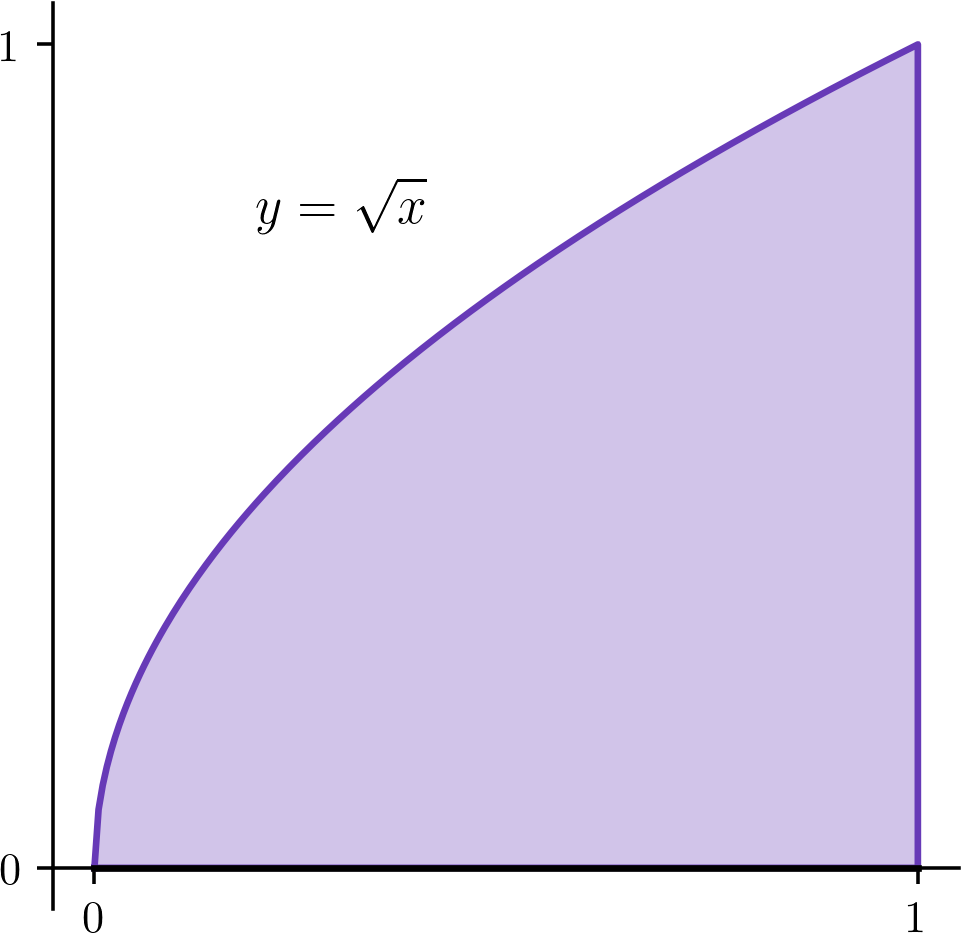
\includegraphics[width=4in]{diskwasher/disk01.png}
\end{image}
\end{center}
\begin{hint}
The radius $R(x)$ will be a difference of $y$-values because slices are indexed by the variable $x$.
Each slice will extend from $y=0$ to $y =  \sqrt{x}$, and so $R(x)$ must be the larger of these $y$-values minus the smaller of these $y$-values.
\end{hint}
\begin{prompt}
\[ R(x) = \answer{\sqrt{x}} \]
\[ V = \int_{\answer{0}}^{\answer{1}} \pi (R(x))^2 dx =  \answer{\frac{\pi}{2}} \]
\end{prompt}
\end{exercise}


\begin{exercise}
The region $0 \leq y \leq \sqrt{x}$ with $x \leq 1$, shown below, is revolved around the axis $x=1$. Use the disk method to find the volume of the solid of revolution.
\begin{center}
\begin{image}
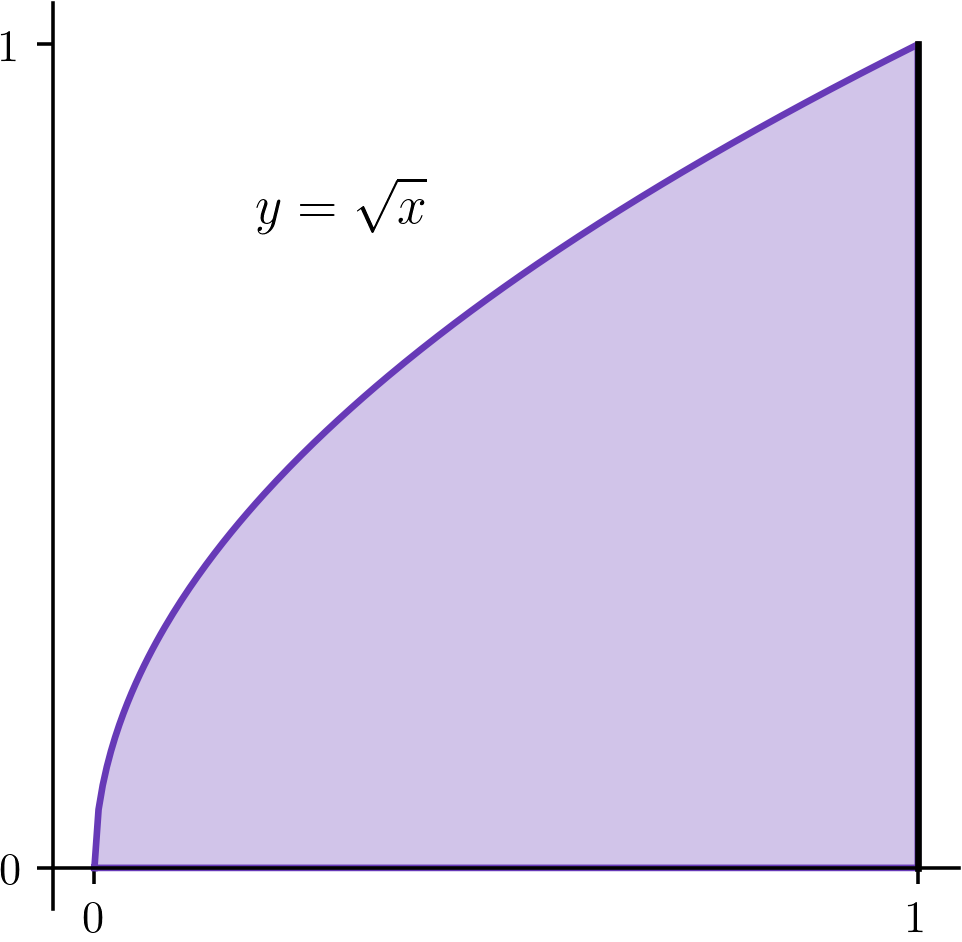
\includegraphics[width=4in]{diskwasher/disk02.png}
\end{image}
\end{center}
\begin{hint}
The radius $R(y)$ will be a difference of $x$-values because slices are indexed by the variable $y$.
Each slice will extend from $x = y^2$ to $x = 1$, and so $R(y)$ must be the larger of these $x$-values minus the smaller of these $x$-values
\end{hint}
\begin{prompt}
\[ R(y) = \answer{1 - y^2} \]
\[ V = \int_{\answer{0}}^{\answer{1}} \pi (R(y))^2 dy = \answer{\frac{8\pi}{15}} \]
\end{prompt}
\end{exercise}


\begin{exercise}
The region $0 \leq y \leq \sqrt{x}$ with $x \leq 1$, shown below, is revolved around the axis $x=0$. Use the washer method to find the volume of the solid of revolution.
\begin{center}
\begin{image}
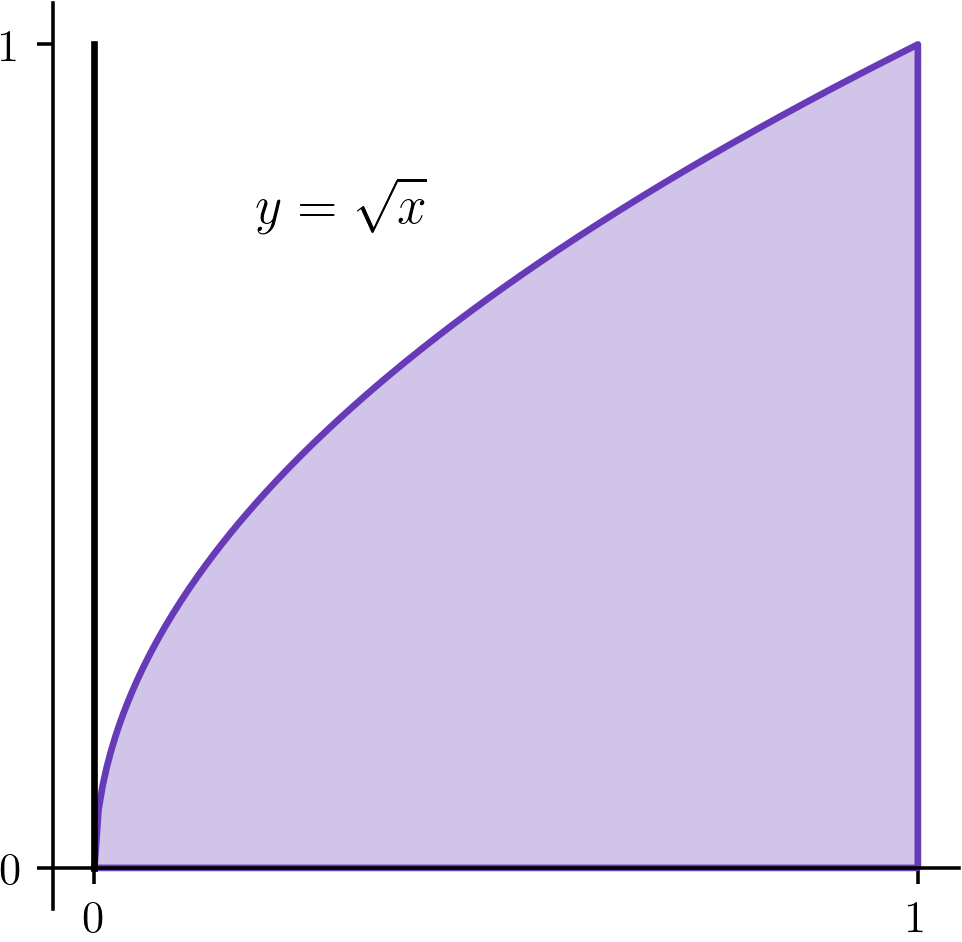
\includegraphics[width=4in]{diskwasher/disk04.png}
\end{image}
\end{center}
\begin{hint}
Each radius will be a difference of $x$-values because slices are indexed by the variable $y$.
The distance from the axis $x=0$ to the line $x=1$ is $1$, and the distance from the axis $x=0$ to $x = y^2$ is $y^2$.
\end{hint}
\begin{prompt}
\[ R_{\mathrm{outer}} (y) = \answer{1} \text{ and } r_{\mathrm{inner}}(y) = \answer{y^2} \]
\[ V = \int_{\answer{0}}^{\answer{1}} \pi  \left[ (R_{\mathrm{outer}}(y))^2 - (r_{\mathrm{inner}}(y))^2 \right] dy =  \answer{\frac{4\pi}{5}} \]
\end{prompt}

\end{exercise}

\begin{exercise}
The region $0 \leq y \leq \sqrt{x}$ with $x \leq 1$, shown below, is revolved around the axis $y=1$. Use the washer method to find the volume of the solid of revolution.
\begin{center}
\begin{image}
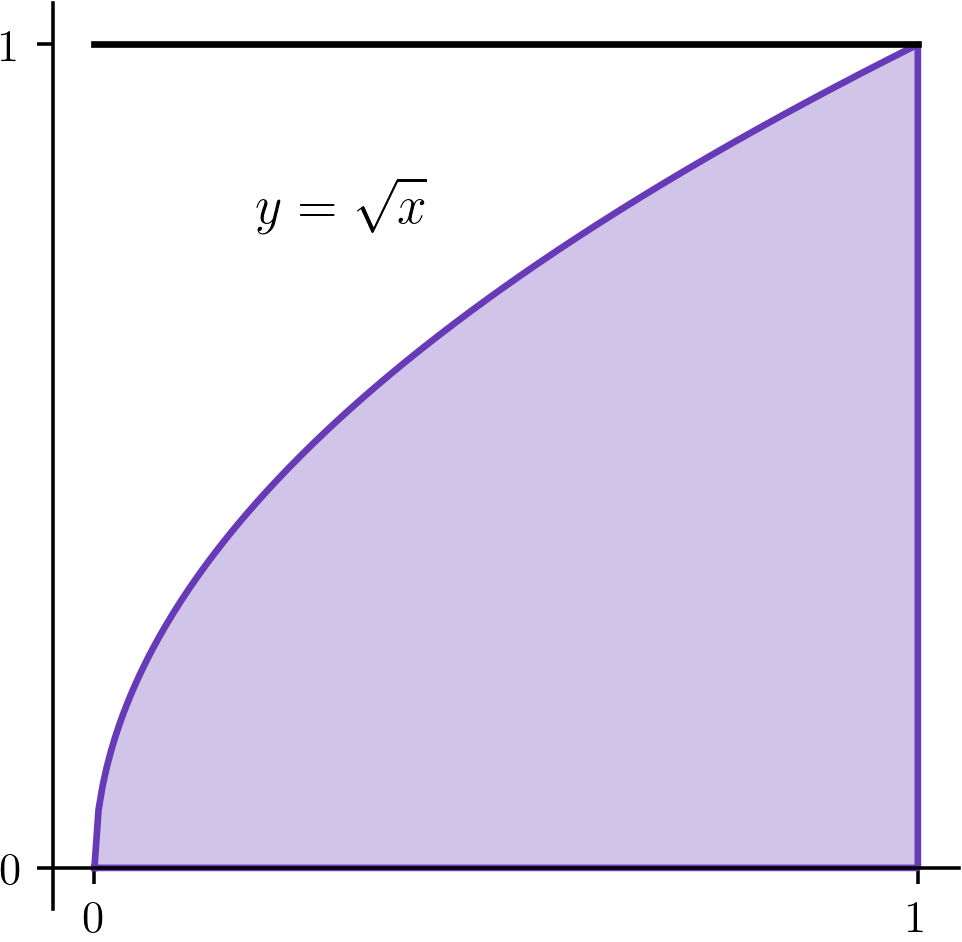
\includegraphics[width=4in]{diskwasher/disk03.png}
\end{image}
\end{center}
\begin{hint}
Each radius will be a difference of $y$-values because slices are indexed by the variable $x$.
The distance from the axis $y=1$ to the line $y=0$ is $1$, and the distance from the axis $y=1$ to $y = \sqrt{x}$ is $1 - \sqrt{x}$.
\end{hint}
\begin{prompt}
\[ R_{\mathrm{outer}} (x) = \answer{1} \text{ and } r_{\mathrm{inner}}(x) = \answer{1-\sqrt{x}} \]
\[ V = \int_{\answer{0}}^{\answer{1}} \pi  \left[ (R_{\mathrm{outer}}(x))^2 - (r_{\mathrm{inner}}(x))^2 \right] dx =  \answer{\frac{5\pi}{6}} \]
\end{prompt}
\end{exercise}



\section*{Sample Quiz Questions}

\begin{question}%%%%%[WasherQuad001]

The region in the plane bounded on the left by the curve \(x=-y^2\), on the right by the curve \(x=y^2+2y+2\), above by the line  \(y = 0\), and below by the line \(y = -2\) is revolved around the axis \(x = 2\). Compute the volume of the resulting solid.
\begin{multiplechoice}
\choice{\(16\pi\)}
\choice{\(20\pi\)}
\choice[correct]{\(24\pi\)}
\choice{\(28\pi\)}
\choice{\(32\pi\)}
\choice{\(36\pi\)}
\end{multiplechoice}
\begin{feedback}
The axis \(x = 2\) is perpendicular to the direction of slices using the integration variable \(y\), which indicates the washer method. 
 The region lies to the left of the axis. One way to see this is to evaluate \(x=-y^2\) at \(y = -2\), giving \(x = -4\), which is to the left of the axis \(x = 2\).
The integral to compute equals \[ \begin{aligned} V &= \int_{-2}^{0}\pi \left((2-(-y^2))^2 - (2-(y^2+2y+2))^2\right)~ dy\\
& = \pi \int_{-2}^{0} (-4y^3+4)~ dy\\
& = \pi \left. \left(-y^4+4y\right) \right|_{-2}^{0} = 24\pi. \end{aligned}\]
\end{feedback}

\end{question}

\begin{question}%%%%%[WasherQuad008]

The region in the plane bounded below by the curve \(y=-2x^2+5x+2\), above by the curve \(y=-2x^2+2x+2\), on the right by the line  \(x = 0\), and on the left by the line \(x = -1\) is revolved around the axis \(y = 2\). Compute the volume of the resulting solid.
\begin{multiplechoice}
\choice[correct]{\(10\pi\)}
\choice{\(14\pi\)}
\choice{\(18\pi\)}
\choice{\(22\pi\)}
\choice{\(26\pi\)}
\choice{\(30\pi\)}
\end{multiplechoice}
\begin{feedback}
The axis \(y = 2\) is perpendicular to the direction of slices using the integration variable \(x\), which indicates the washer method. 
 The region lies below the axis. One way to see this is to evaluate \(y=-2x^2+5x+2\) at \(x = -1\), giving \(y = -5\), which is below the axis \(y = 2\).
The integral to compute equals \[ \begin{aligned} V &= \int_{-1}^{0}\pi \left((2-(-2x^2+5x+2))^2 - (2-(-2x^2+2x+2))^2\right)~ dx\\
& = \pi \int_{-1}^{0} (-12x^3+21x^2)~ dx\\
& = \pi \left. \left(-3x^4+7x^3\right) \right|_{-1}^{0} = 10\pi. \end{aligned}\]
\end{feedback}

\end{question}

\begin{question}%%%%%[washersqrtsub001]

The region in the plane given by \(\left|{- \frac{x}{2} + \frac{1}{2} \sqrt{9 - 6 x^{2}}}\right| \leq y \leq \frac{x}{2} + \frac{1}{2} \sqrt{9 - 6 x^{2}}\) and \(0 \leq x \leq \frac{2}{3} \sqrt{3}\) is revolved around the \(x\)-axis. Compute the volume of the resulting solid.
\begin{multiplechoice}
\choice[correct]{\(\displaystyle \frac{13}{9} \pi\)}
\choice{\(\displaystyle \frac{19}{9} \pi\)}
\choice{\(\displaystyle \frac{26}{9} \pi\)}
\choice{\(\displaystyle \frac{28}{9} \pi\)}
\choice{\(\displaystyle \frac{37}{9} \pi\)}
\choice{\(\displaystyle \frac{49}{9} \pi\)}
\end{multiplechoice}
\begin{feedback}
If the variable \(x\) is used for slicing, then slices are perpendicular to the axis of rotation, which indicates the washer method should be used.
The inequalities for \(y\) give the outer and inner radii, and \[ \left(\frac{x}{2} + \frac{1}{2} \sqrt{9 - 6 x^{2}}\right)^2 - \left( \left|{- \frac{x}{2} + \frac{1}{2} \sqrt{9 - 6 x^{2}}}\right|\right)^2 = x \sqrt{9 - 6 x^{2}}. \](Note that the absolute values go away when the radius is squared.)To compute the integral 
\[ \int_{0}^{\frac{2}{3} \sqrt{3}} \pi x \sqrt{9 - 6 x^{2}}\, dx \]
 we can use the substitution \(u = 9 - 6 x^{2}\) which implies the equality \(du = \left(- 12 x\right)dx\) for the differentials. This gives the equality
\[ \begin{aligned} \int \pi x \sqrt{9 - 6 x^{2}}\, dx & = \int \left(- \frac{\pi}{12} \sqrt{u}\right)\, du \\
 & = - \frac{\pi}{18} u^{\frac{3}{2}}. \end{aligned} \]
Reversing the substitution gives
\[ \begin{aligned} \int_{0}^{\frac{2}{3} \sqrt{3}} \pi x \sqrt{9 - 6 x^{2}}\, dx & = \left. \left[- \frac{\pi}{18} \left(9 - 6 x^{2}\right)^{\frac{3}{2}} \right] \right|_{0}^{\frac{2}{3} \sqrt{3}}\\ & = \left(- \frac{\pi}{18} \right) - \left(- \frac{3}{2} \pi \right) = \frac{13}{9} \pi. \end{aligned} \]
\end{feedback}

\end{question}


\end{document}
